\chapter{Implementierung}

\section{Scanner Konstruktion}
Um das Lichtschnittverfahren angemessen umsetzen zu können, müssen zuerst brauchbare Daten erhoben werden. Mit Daten sind in diesem Kontext die Fotografien gemeint, auf denen das zu vermessende Objekt inklusive der projizierten Laserlinie zu sehen ist. Um diese Reihe von Bildern zu erstellen, ist eine Vorrichtung von Nöten, die es ermöglicht, die Webcam und den Laser so zu fixieren, dass das zu vermessene Objekt mit Leichtigkeit fotografierbar ist. Zusätzlich müssen sowohl der Laser als auch die Kamera so beweglich sein, dass das zu vermessene Objekt in kontrollierten Abständen mit dem Laser abgetastet werden kann, sich das räumliche Verhältnis zwischen Webcam und Laser sich jedoch nicht verändert. 

Für das vorliegende Projekt wurde versucht, dies unter Berücksichtigung einer einfachen und günstigen Konstruktion zu realisieren. Die in dieser Ausarbeitung vorgeschlagene Lösung setzt darauf, Kamera und Laser übereinander auf einer Pappelholzplatte zu fixieren. Diese Holzplatte befindet sich auf zum Boden senkrecht befindlichen Schlaufen aus stabilem Gurt, welche um zwei PVC-Röhren gespannt sind. Besagte PVC-Röhren ruhen in horizontaler Lage parallel zum Boden in zwei Holzstreben, welche wiederrum senkrecht auf einer Basis aus dünnem Pappelholz geklebt sind. Die Gesamtkonstruktion kann in Abb. \ref{fig:scanner1} und \ref{fig:scanner2} und betrachtet werden.

\begin{figure}
\centering
\begin{minipage}{0.45\textwidth}
\centering 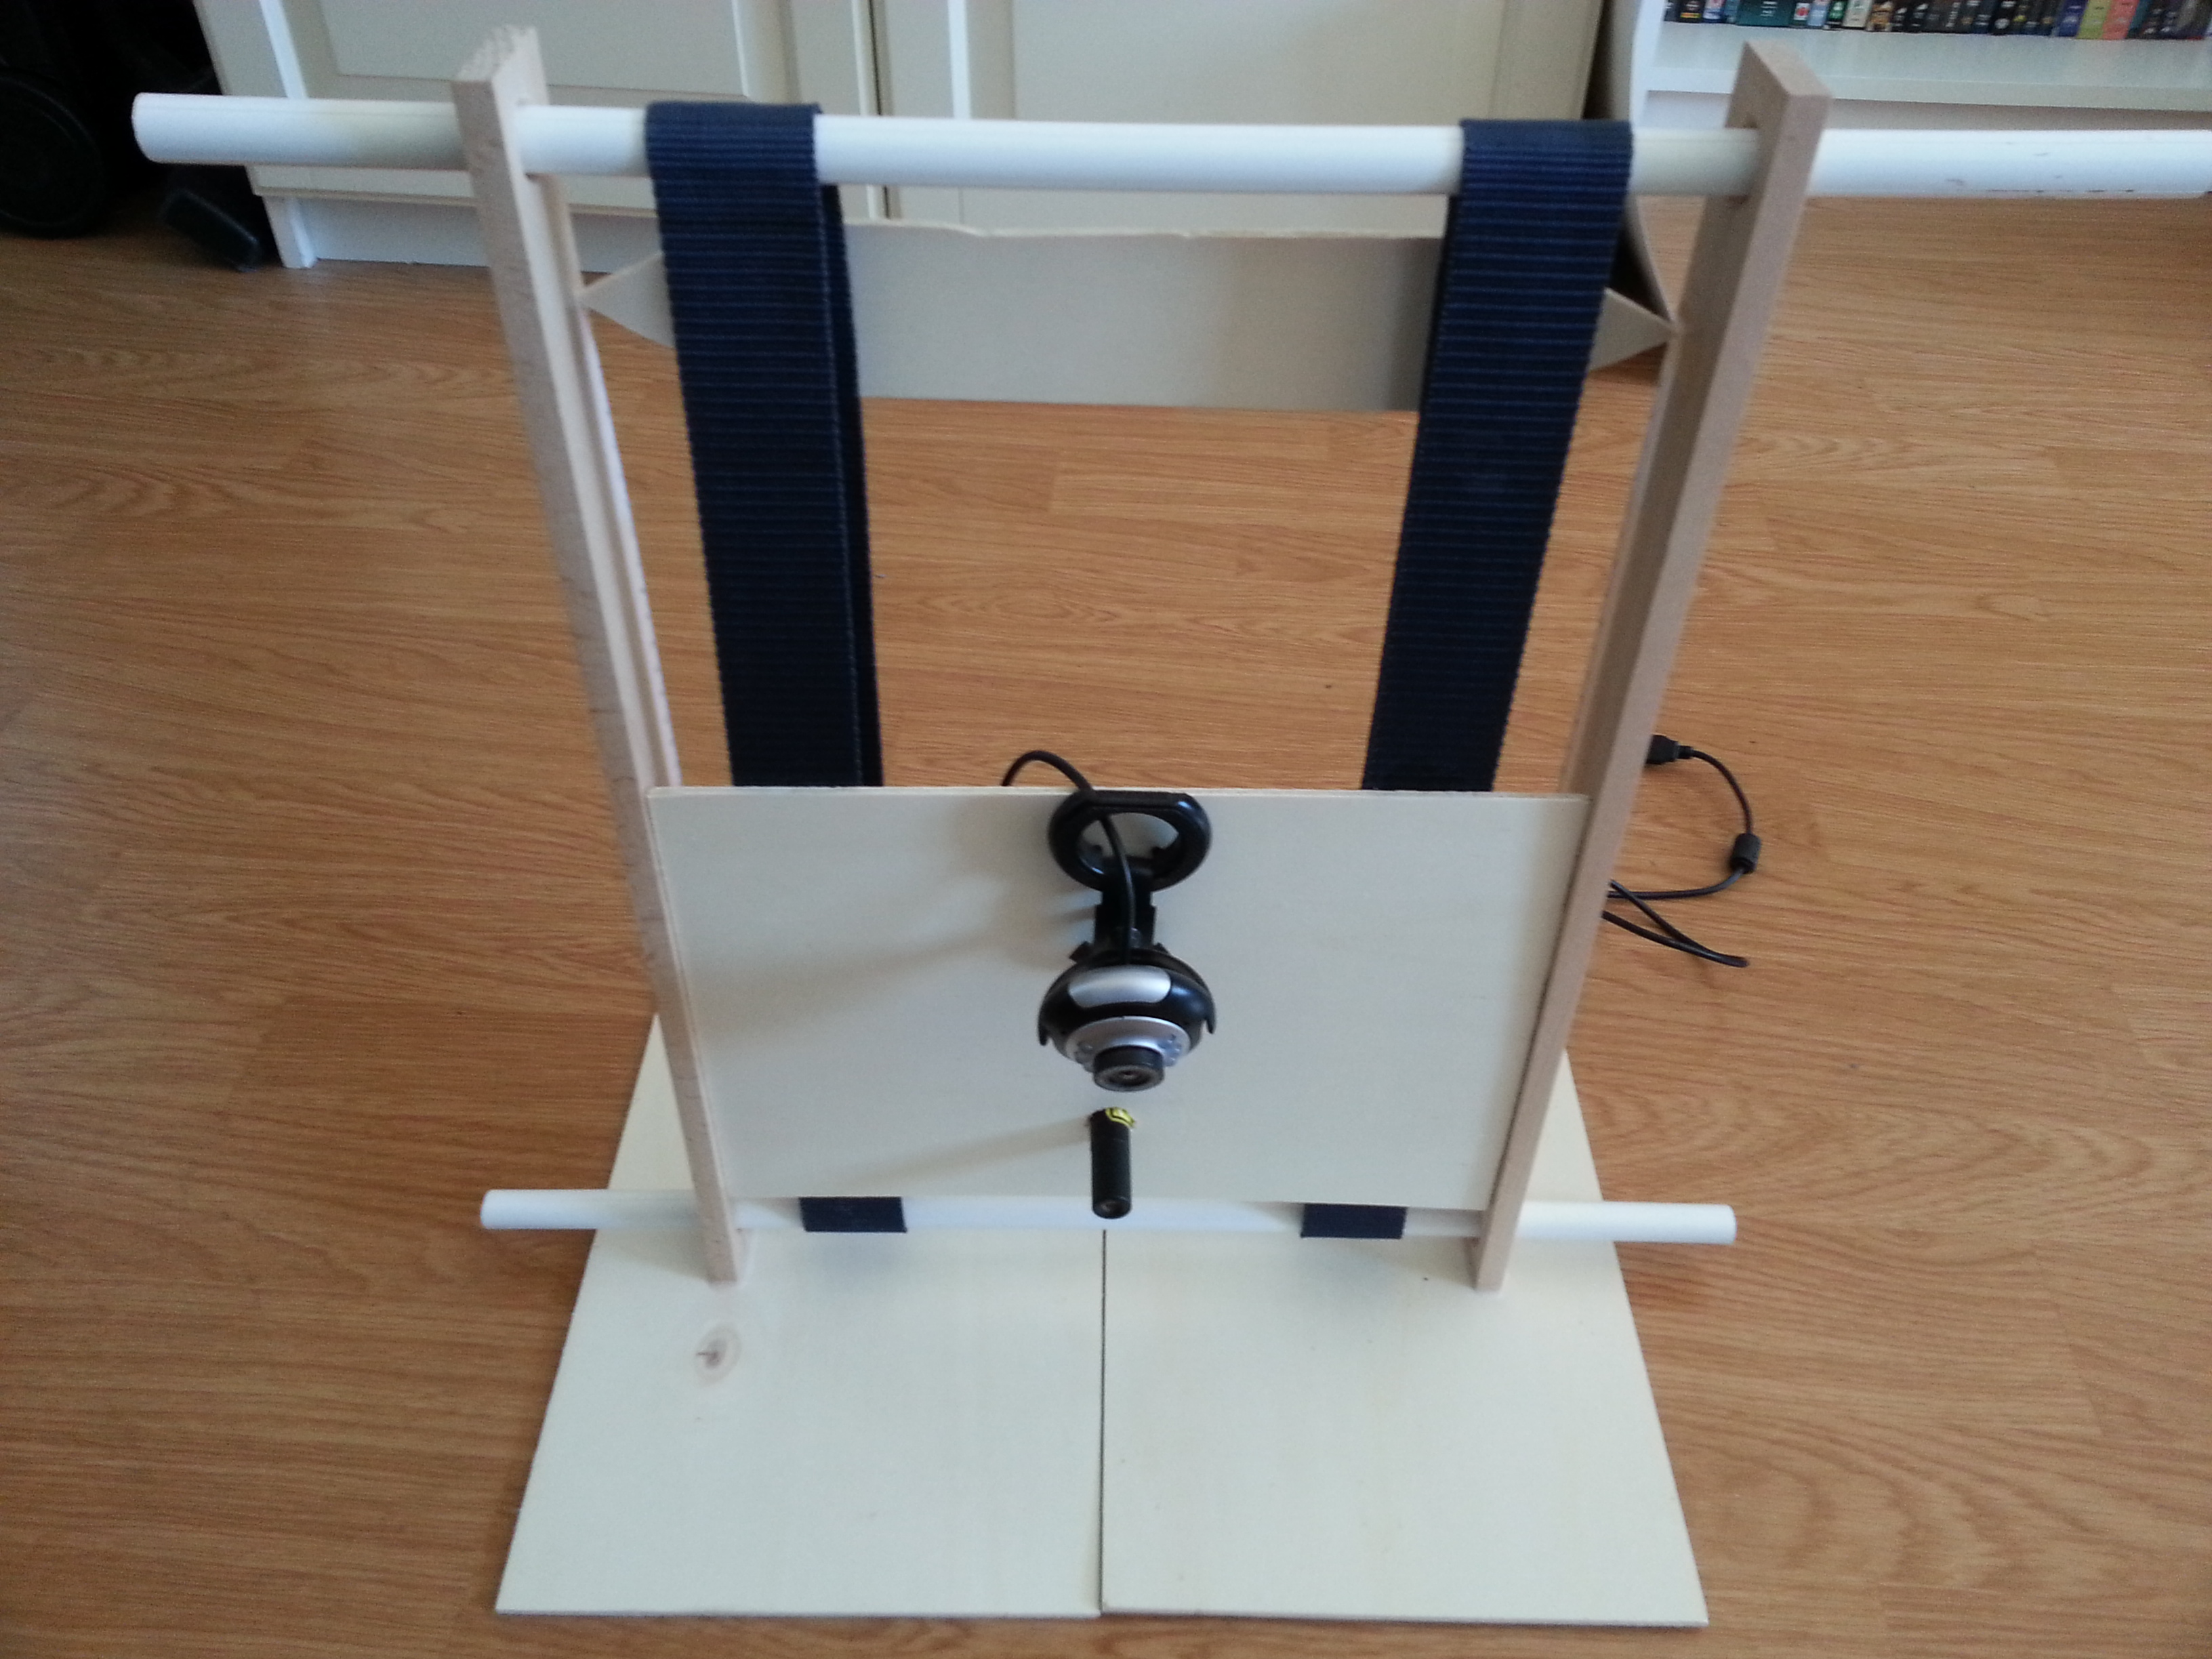
\includegraphics[width=\textwidth]{images/Scanner1.jpg}\label{fig:scanner1}
\caption{Frontal Ansicht}
\end{minipage}
\begin{minipage}{0.45\textwidth}
\centering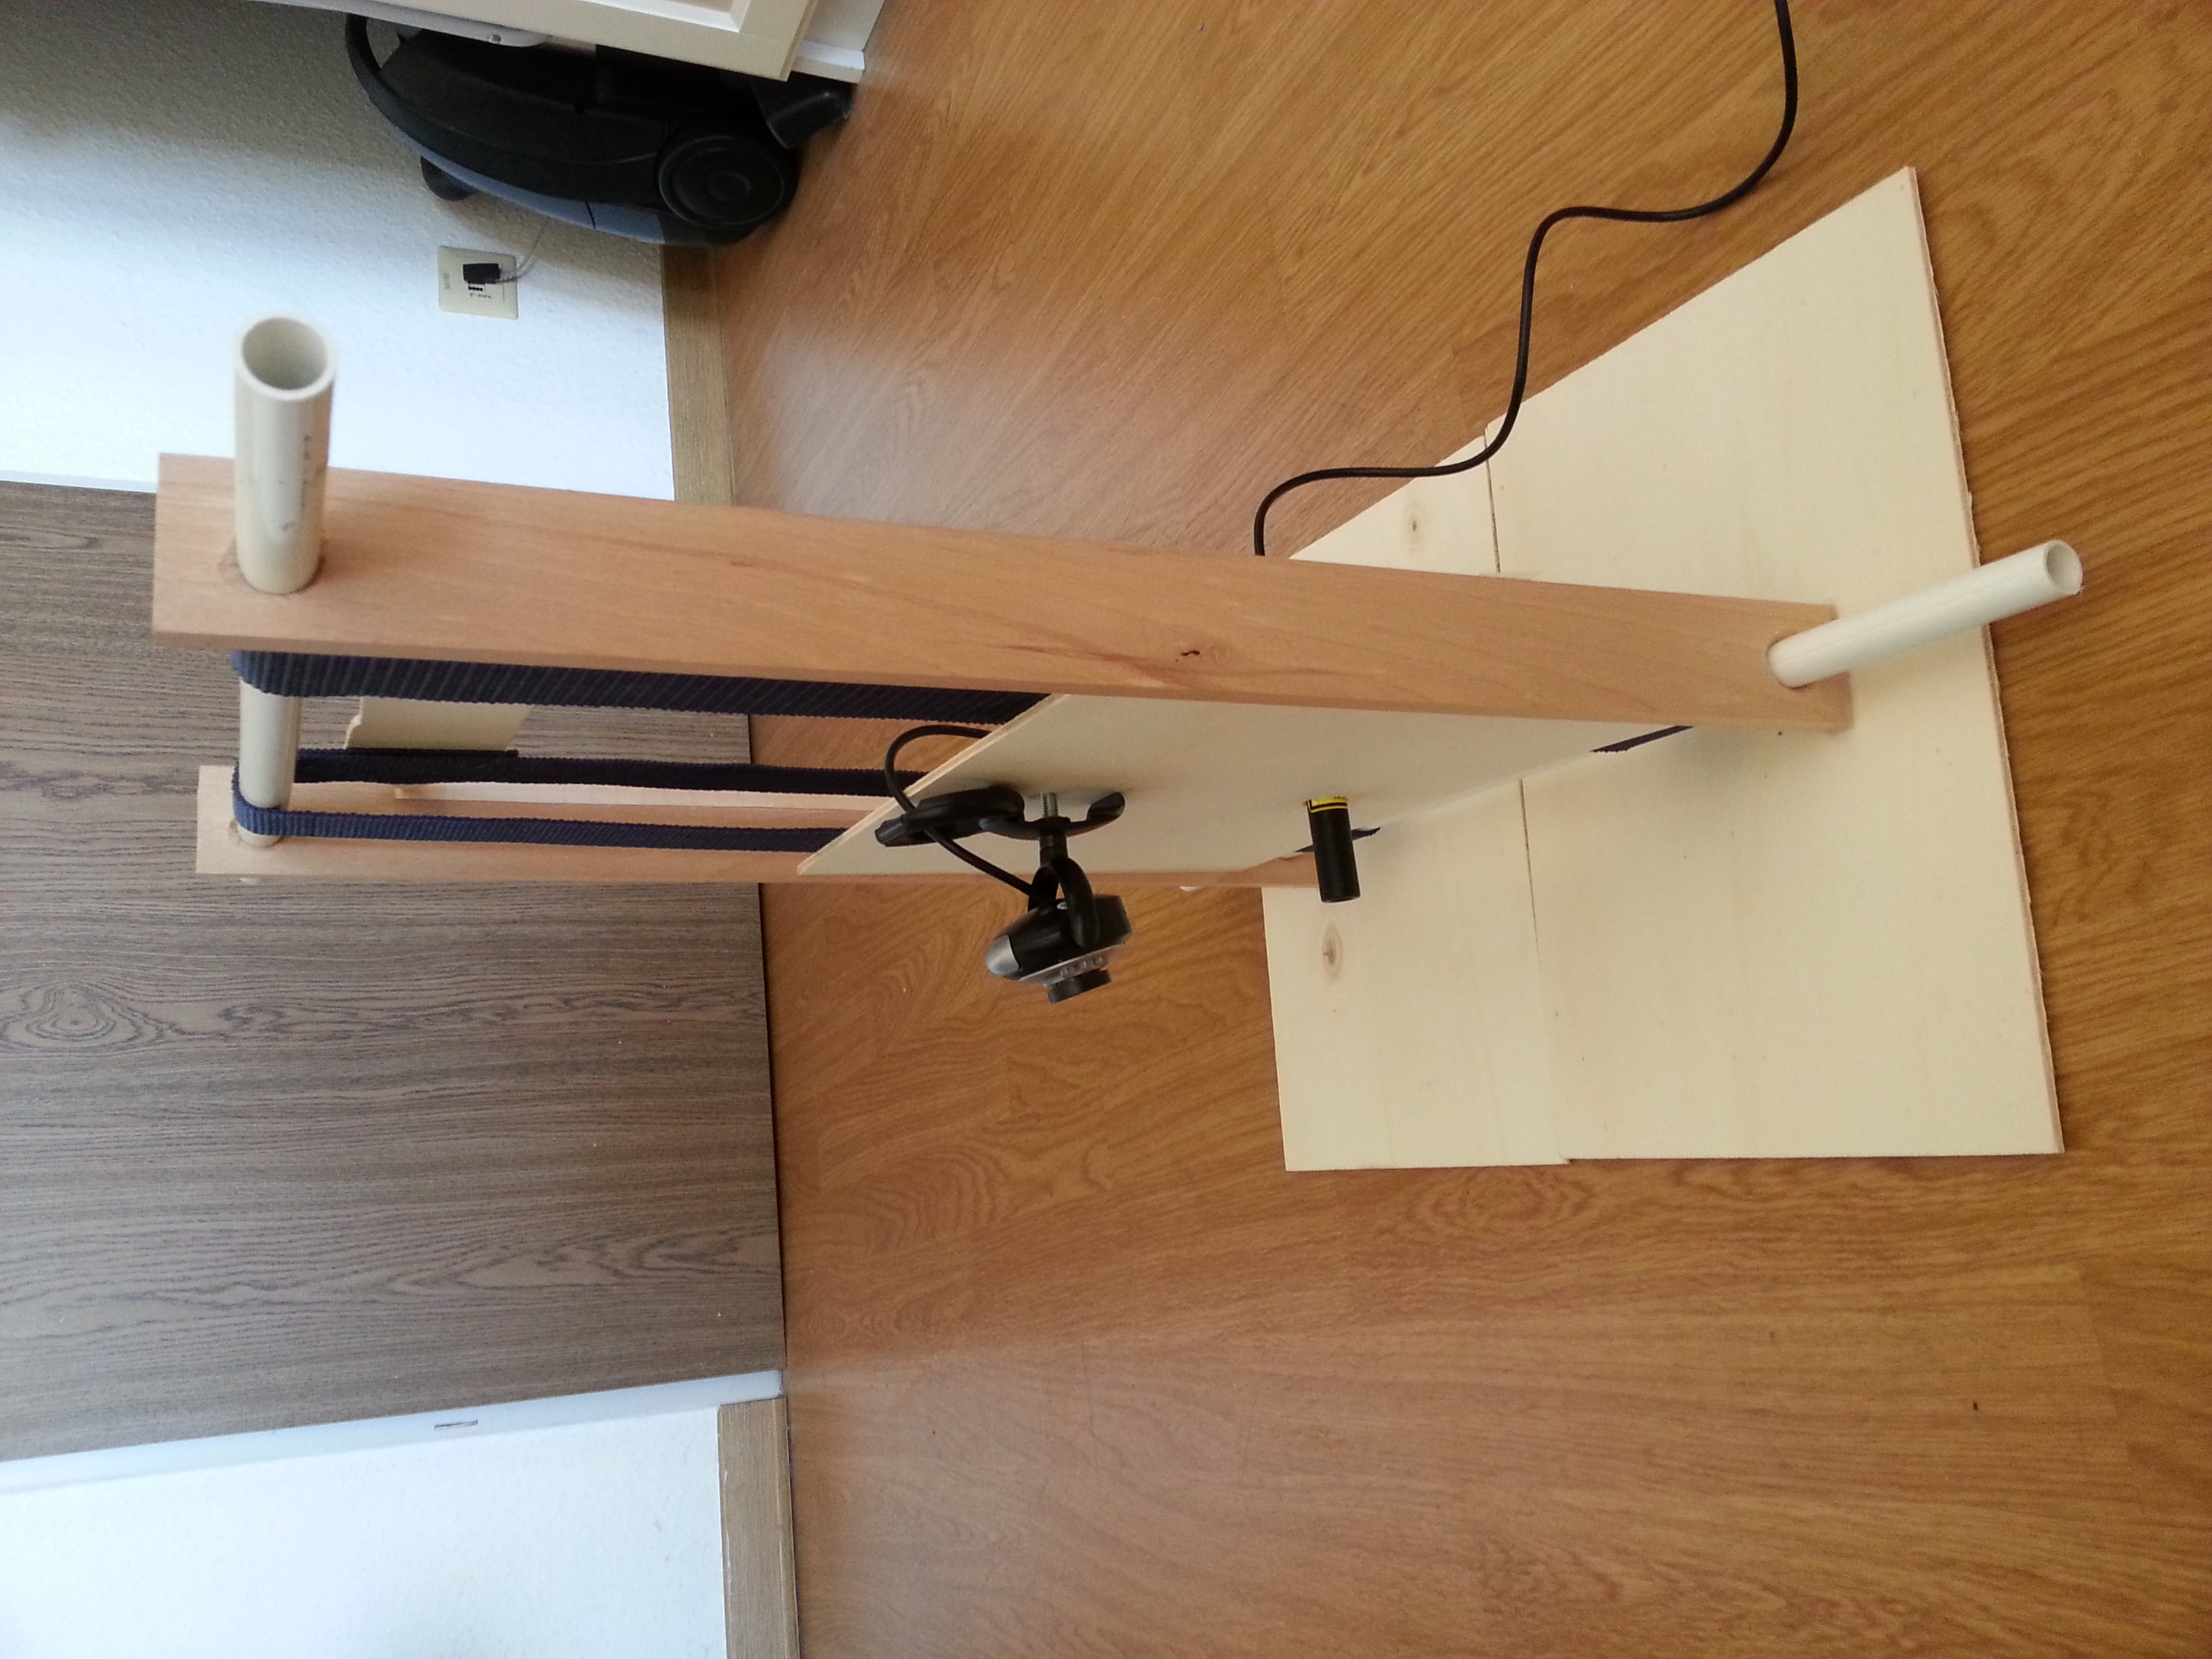
\includegraphics[width=\textwidth, angle = -90]{images/Scanner2.jpg}\label{fig:scanner2}
\caption{Seitliche Ansicht}
\end{minipage}
\end{figure}

\begin{figure}
\centering 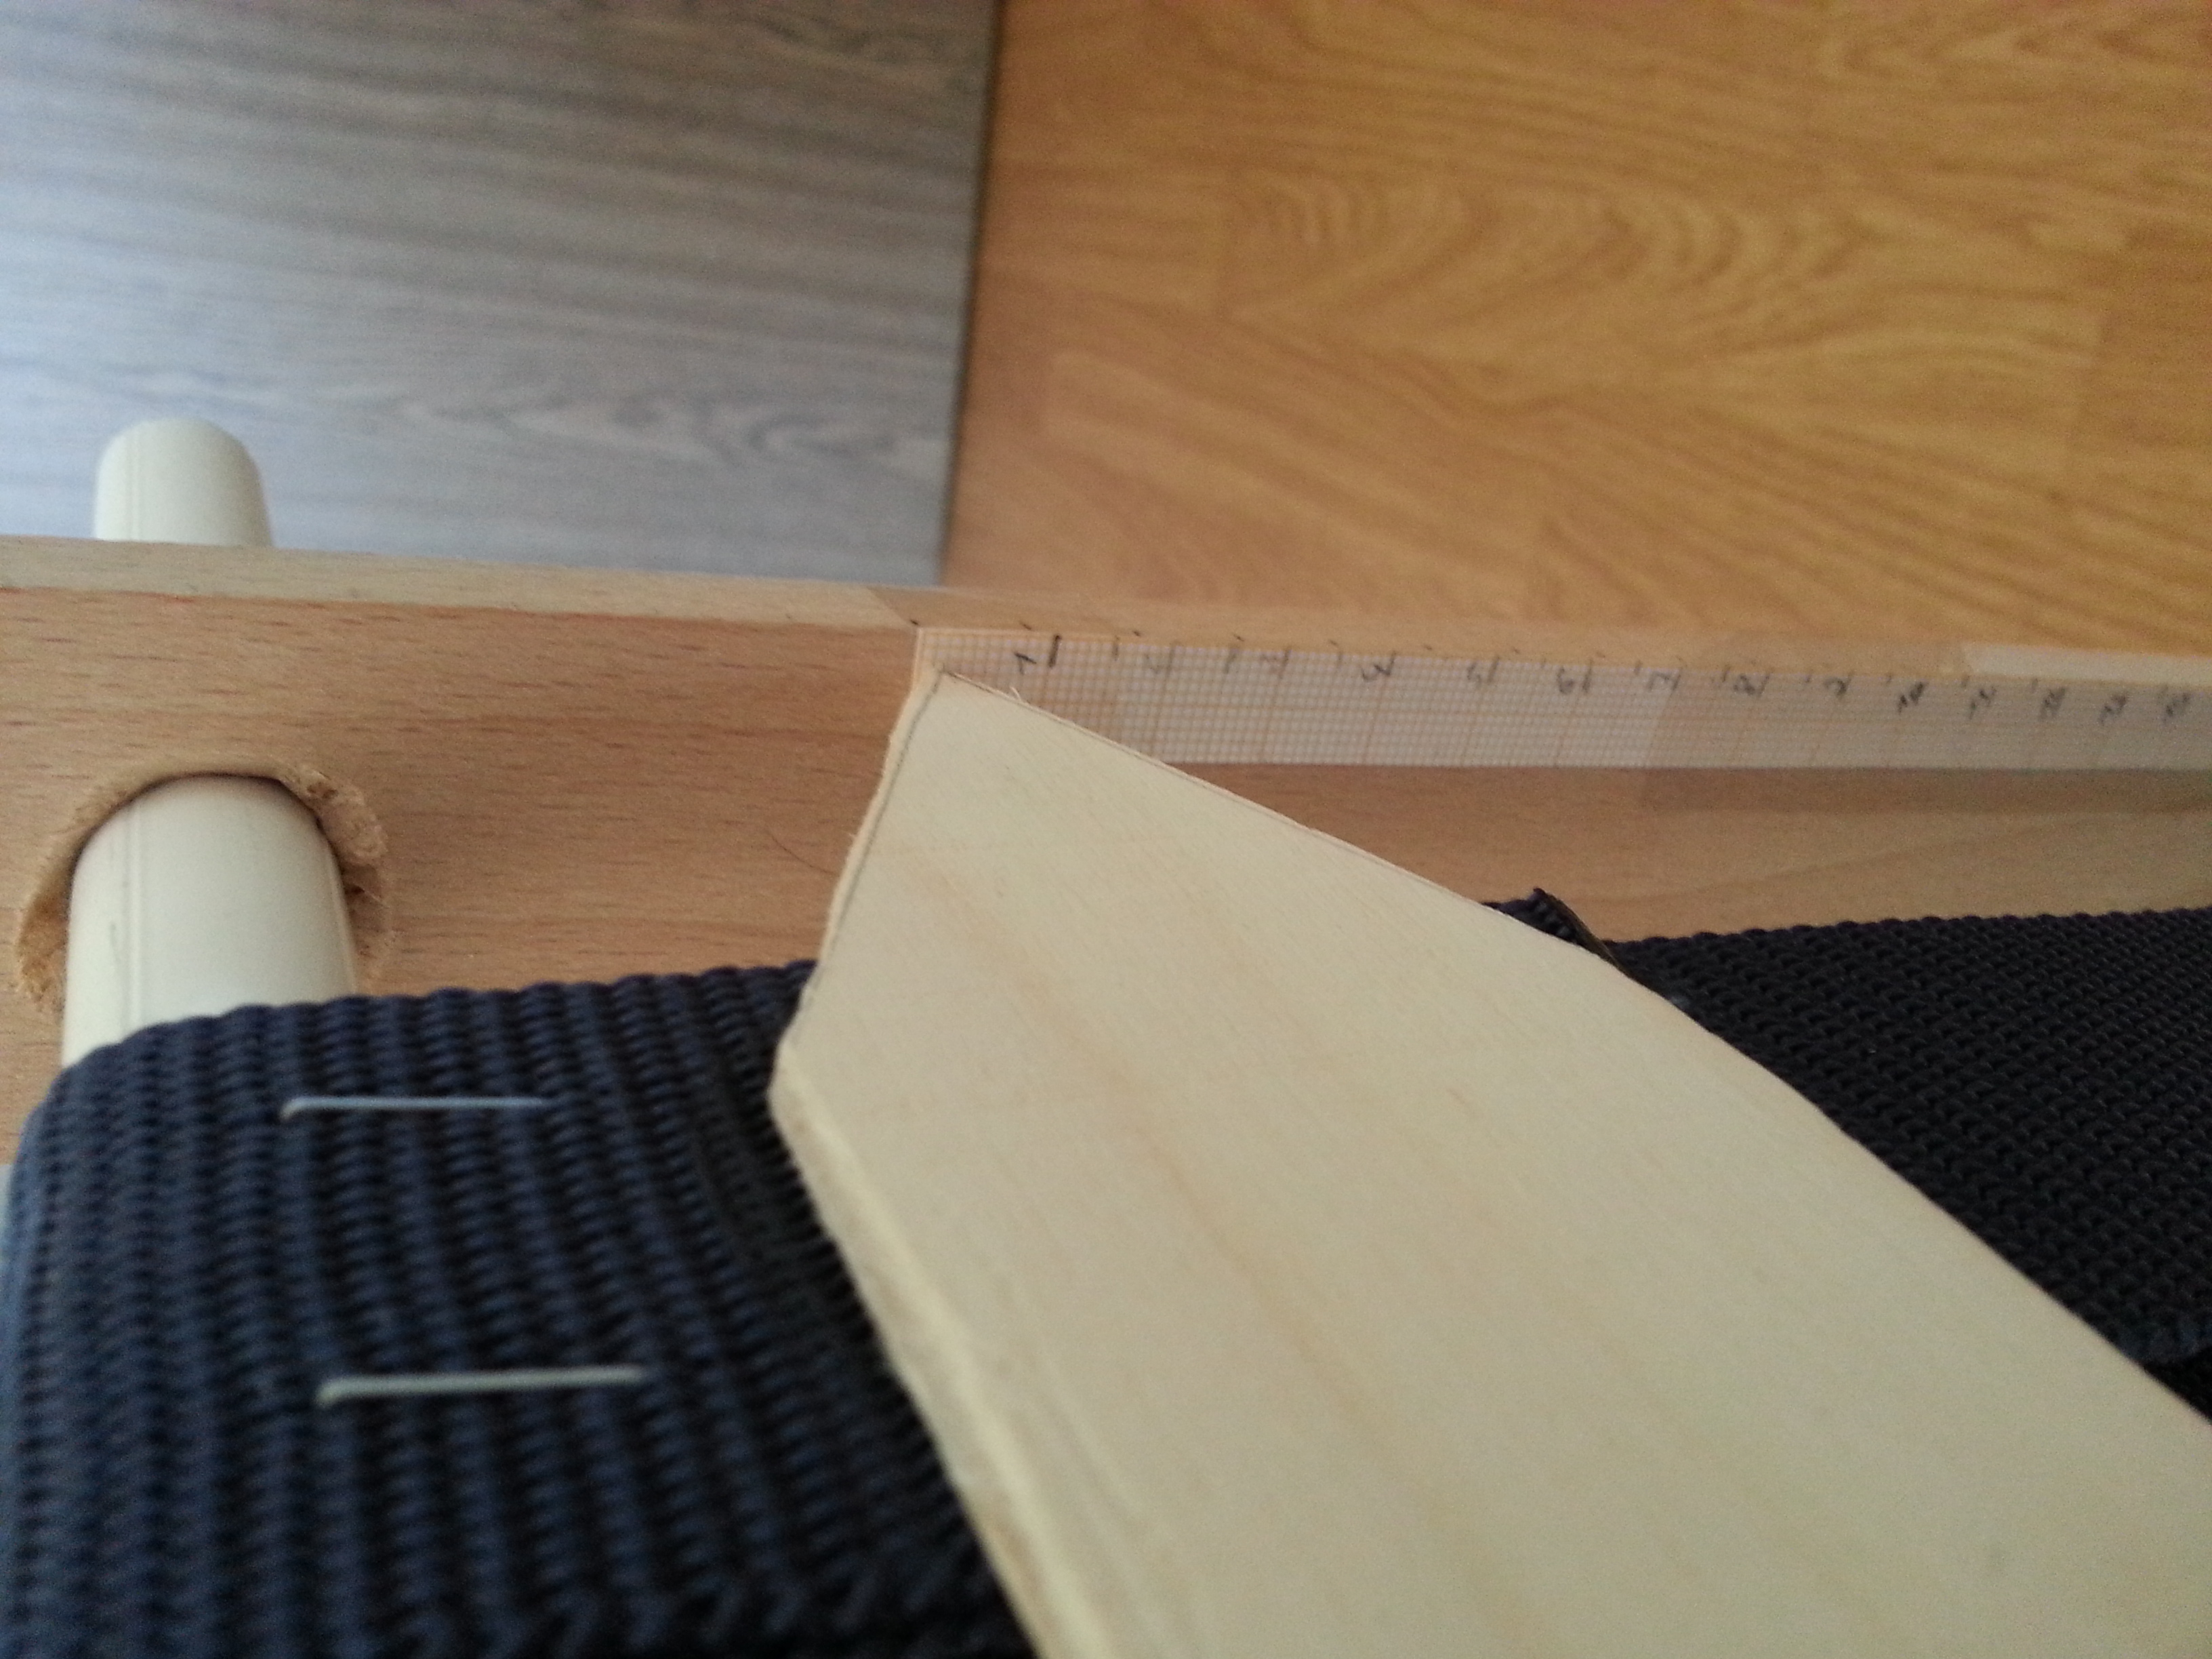
\includegraphics[width=0.5\textwidth, angle = -90]{images/Scanner3.jpg}\label{fig:scanner3}
\caption{Nahaufnahme der Millimeter-Anzeige}
\end{figure}

Die vom Laser aufgespannte Ebene befindet sich somit parallel zum Grund, während die Kamera schräg von oben auf das zu vermessene Objekt schaut. Mittels des Gurts kann die Holzplatte, auf der Kamera und Laser montiert sind, von unten nach oben bewegt werden, um das Objekt so abzutasten. Um zu kontrollieren, wie weit der Laser über das Objekt bewegt wurde, ist auf der Rückseite des Gurts eine Anzeige installiert, welche sich gen Boden bewegt sobald Laser und Kamera nach oben steigen. Die Anzeige zeigt an den Seiten der Holzstreben, an denen eine Skala in Millieter-Papier angebracht ist, wie weit sich die Holzplatte von der Startposition aus nach oben bewegt hat. In Abb. \ref{fig:scanner3} ist eine Nahaufnahme dieser Anzeige zu sehen.

Ein wesentlicher Vorteil der vorgenommenen Konstruktion liegt in der Parallelität der Laser-Ebene zum Boden. Auf diese Weise muss man sich bei der späteren Bildverarbeitung keine Sorgen machen, dass die Laser-Linie auf den Untergrund fällt, auf dem das zu vermessene Objekt ruht. Wäre dies der Fall, müssten bei der späteren Auslesung die Teile der Laser-Linie, die auf das Objekt fallen, von denen, die auf den Untergrund fallen, aufwendig getrennt werden. Ebenfalls macht der Aufbau die Nachbearbeitung der gemessenen Weltkoordinaten im Gegensatz zu vergleichbaren Konstruktionen (z.B. bei schwenkbaren Scannern) besonders simpel: Da sich die Apparatur zwischen Aufnahmen lediglich entlang der Z-Achse bewegt und dieser Abstand bekannt ist, kann auf den Z-Achsen-Anteil des Messungsendergebnis der besagte Abstand einfach addiert werden.

Der Gesamtaufbau setzt vor allem auf eine praktikable Lösung, die problemlos nachgebaut werden kann und sich dem zu Grunde liegenden Problem so nähert, dass anschließende Verarbeitungen und Berechnungen erleichtert werden. Zudem ist die Konstruktion kostengünstig. In Tabelle \ref{tab:preise} können die Preise in Euro eingesehen werden, die alle Komponenten (außer Kleinteile wie einzelne Schrauben, Holzleim etc.) gekostet haben. Zusammen kommt der Scanner auf einen Preis von ca. 45,14\euro

\begin{table} %[hbtp]
	\centering
		\begin{tabular}{l | l}
		\textbf{Komponente} & \textbf{Preis in Euro}\\
		\hline
			Kamera "`TeckNet C016 USB HD Webcam"' & 13,99 \euro\\
			Linienlaser &  ca. 20 \euro\\
			PVC-Röhre & 1,69 \euro\\
			Holzleiste Buche (Seitenstreben) & 3,79 \euro\\
			Pappel-Sperrholz &  2,29 \euro\\
			Gurtband & 3,38 \euro
		\end{tabular}
	\caption{Bezeichnung der Tabelle}
	\label{tab:preise}
\end{table}


\section{Der Scanvorgang}
\begin{figure}
\centering 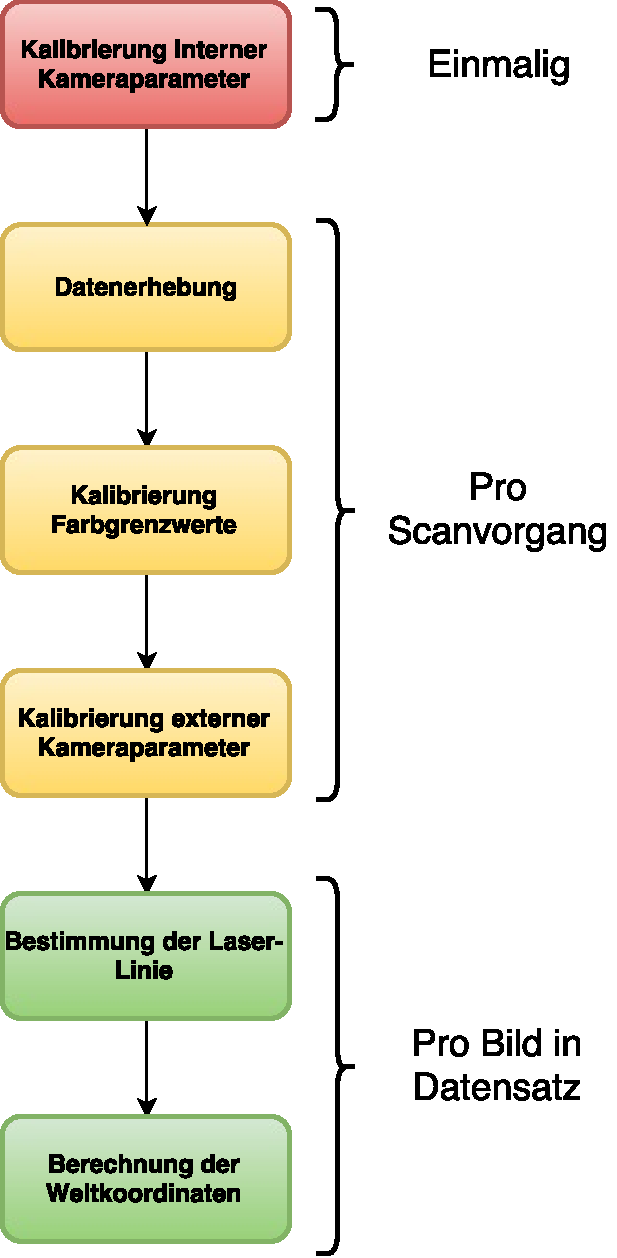
\includegraphics[width=1.0\textwidth]{images/ScannerVerfahren.pdf}\label{fig:scanVorgang}
\caption{Der schematische Ablauf des Scanvorgangs}
\end{figure}

\subsection{Datenerhebung}
TODO

\subsection{Kalibrierung und weitere Vorbereitungen}
TODO

\subsection{Datenverarbeitung}
TODO

\subsubsection{Lokalisierung der Laserlinie}
TODO

\subsubsection{Berechnung der Weltkoordinaten}
TODO

